\documentclass{article}

\usepackage{amsmath, amsthm, amssymb, amsfonts}
\usepackage{thmtools}
\usepackage{graphicx}
\usepackage{setspace}
\usepackage{geometry}
\usepackage{float}
\usepackage{hyperref}
\usepackage[utf8]{inputenc}
\usepackage[english]{babel}
\usepackage{framed}
\usepackage[dvipsnames]{xcolor}
\usepackage{tcolorbox}

\usepackage{physics}
\usepackage[outline]{contour}
\usepackage{tikz}

\usetikzlibrary{angles,quotes} % for pic
\usetikzlibrary{bending} % for arrow head angle
\contourlength{1.0pt}
\usetikzlibrary{3d}

\tikzset{>=latex} % for LaTeX arrow head
\colorlet{myblue}{blue!65!black}
\colorlet{mydarkblue}{blue!50!black}
\colorlet{myred}{red!65!black}
\colorlet{mydarkred}{red!40!black}
\colorlet{veccol}{green!70!black}
\colorlet{vcol}{green!70!black}
\colorlet{xcol}{blue!85!black}

\tikzstyle{vector}=[->,very thick,xcol,line cap=round]
\tikzstyle{xline}=[myblue,very thick]
\tikzstyle{yzp}=[canvas is zy plane at x=0]
\tikzstyle{xzp}=[canvas is xz plane at y=0]
\tikzstyle{xyp}=[canvas is xy plane at z=0]
\def\tick#1#2{\draw[thick] (#1) ++ (#2:0.12) --++ (#2-180:0.24)}
\def\N{100}

\colorlet{LightGray}{White!90!Periwinkle}
\colorlet{LightOrange}{Orange!15}
\colorlet{LightGreen}{Green!15}
\colorlet{LightPurple}{Purple!15}
\colorlet{LightDandelion}{Dandelion!15}


\newcommand{\HRule}[1]{\rule{\linewidth}{#1}}

\declaretheoremstyle[name=Teorema,]{thmsty}
\declaretheorem[style=thmsty,numberwithin=section]{theorem}
\tcolorboxenvironment{theorem}{colback=LightGray}

\declaretheoremstyle[name=Proposición,]{prosty}
\declaretheorem[style=prosty,numberlike=theorem]{proposition}
\tcolorboxenvironment{proposition}{colback=LightOrange}

\declaretheoremstyle[name=Definición,]{prcpsty}
\declaretheorem[style=prcpsty,numberlike=theorem]{definition}
\tcolorboxenvironment{definition}{colback=LightGreen}

\declaretheoremstyle[name=Ejercicio,]{xrcsty}
\declaretheorem[style=xrcsty,numberlike=theorem]{exercise}
\tcolorboxenvironment{exercise}{colback=LightDandelion}

\setstretch{1.2}
\geometry{
    textheight=9in,
    textwidth=5.5in,
    top=1in,
    headheight=12pt,
    headsep=25pt,
    footskip=30pt
}

\newcommand{\Nat}{\mathbb{N}}
\newcommand{\C}{\mathbb{C}}
\newcommand{\R}{\mathbb{R}}
\newcommand{\Phisub}[1]{$\varphi_#1$}
\newcommand{\CuerpoC}{(\C, +,\cdot)}
\newcommand{\matriz}[4]{\begin{pmatrix}
#1 & #2\\
#3 & #4
\end{pmatrix}}


\providecommand{\norm}[1]{\lVert#1\rVert}

% ------------------------------------------------------------------------------

\begin{document}

% ------------------------------------------------------------------------------
% Cover Page and ToC
% ------------------------------------------------------------------------------

\title{ \normalsize \textsc{}
		\\ [2.0cm]
		\HRule{1.5pt} \\
		\LARGE \textbf{\uppercase{Compleja}
		\HRule{2.0pt} \\ [0.6cm] \LARGE{Universidad de Murcia}}\\
        %\vspace{12pt} % Whitespace
	    %\rule{\linewidth}{2pt}\\ % Thick bottom horizontal rule
	    %\vspace{12pt} % Whitespace
	    \includegraphics[scale=0.25]{floresportada.png}
		}
\date{\normalsize\today}
\author{\textbf{Author} \\ 
		Alonso Oma Alonso \\
		Murcia}

\maketitle
\newpage

\tableofcontents
\newpage

% ------------------------------------------------------------------------------

\begin{section}{Tema 1:}

    \begin{subsection}{El cuerpo $\mathbb{C}$ de los números complejos}
        Historicamente, un número complejo es $a+i\cdot b$, donde a, b $\in \mathbb{R}$, y donde el símbolo $i$
        cumple $i^2 = -1$.

        Usando esta regla se define un producto formal
        \[(a+ib)\cdot(c+id) = a\cdot(c+id) + ib\cdot(c+id)=ac+iad+ibc+i^2bd=(ac-bd)+i(ad+bc)\]

        \begin{definition}
            Llamamos $\mathbb{C}$ al conjunto $\mathbb{R}^2 = \{(a,b)\ |\ a,b\in \mathbb{R}\}$ dotado con las reglas de
            composición 
            \begin{itemize}
                \item \textbf{Suma:} $(a,b) + (a',b') = (a+a', b+b')$
                \item \textbf{Producto:} $(a,b) \cdot (c,d) = (ac-bd, ad+bc)$
            \end{itemize}       
        \end{definition}

        Denotaremos $i\equiv (0,1)\in \mathbb{C}$, y si $a\in \mathbb{R}\Rightarrow a\equiv(a,0)$.

        En Particular, \[a+ib = (a,0) + (0,1)\cdot (b,0) \overbrace{=}^{PROD} (a,0) + (0,b)=(a,b)\]
        \[i^2 = (0,1)\cdot (0,1)=(-1,0) = -1\]
        Así los elementos $z=(a,b)\in \C$ se identifican con $a+ib$.


        \begin{theorem}
            $(\C, +,\cdot)$ es un cuerpo conmutativo tal que
            \begin{itemize}
                \item contiene a $\mathbb{R}\equiv \mathbb{R}\times \{0\}$ como subcuerpo
                \item $z^2=-1$ tiene solución
            \end{itemize}
            Además, es el menor cuerpo con esas dos propiedades.
        \end{theorem}
        \begin{proof}
            Ejercicio sencillo de álgebra:
            \begin{itemize}
                \item $(\C, +)$ es grupo abeliano.
                \item $(\C/\{0\}, \cdot)$ es grupo abeliano.
                \item Propiedad distributiva.
            \end{itemize}

            La única propiedad no trivial es $z\in \C/\{0\}\Longrightarrow\exists z^{-1}\in\C | z\cdot z^{-1} = z^{-1}\cdot z = 1.$
            
            Para probarlo hallamos $z^{-1} = \frac{1}{a+ib}$ formalmente: $z^{-1} = (a+ib)(a-ib) = \frac{a}{a^2+b^2} -i\frac{b}{a^2+b^2} = (\frac{a}{a^2+b^2}, \frac{-b}{a^2+b^2})\in \C$.

            Con esta expresión explícita se comprueba que $z\cdot z^{-1} = 1$.
            \begin{itemize}
                \item Claramente $\C$ contiene a $\mathbb{R} = \{(a,0)|a\in \mathbb{R}\}$, y la ecuación $z^2 = -1$ tiene solución en $\C: \ z=\pm i=(0,\pm 1)\in\C$
                \item Además, cualquier otro cuerpo con esas propiedades debe contener $a+bi, \forall a,b \in \R \Rightarrow \C \subseteq \mathbb{K}$.
            \end{itemize}
        \end{proof}

        \begin{exercise}
            Si $w\in \C$, probar que $\exists \ z\in \C $ tal que $ \ z^2 = w$.
            
            \textbf{Sugerencia:} Escribir $w=a+ib$,  buscar $z=x+iy$ tal que $(x+iy)^2 = a+ib$.
        \end{exercise}
        \begin{exercise}\hfil
            \begin{itemize}
                \item Operar $\frac{1}{4+4i},\ \sqrt{3+4i}, \ (1+i)^4$
                \item Probar que $\CuerpoC$ no admite ningún orden total.
            \end{itemize}
        \end{exercise}
        \begin{definition}
            Si $z=a+ib \in \C$, definimos 
            \begin{itemize}
                \item \textbf{Parte real:} $Re(z)=a$
                \item \textbf{Parte imaginaria:} $Im(z) = b$
                \item \textbf{Módulo:} $|z|^2 := \sqrt{a^2+b^2}$
                \item \textbf{Conjugado:} $\overline{z}:= a-ib$
            \end{itemize}
            Notar que $Re(z) = \frac{z+\overline{z}}{2}$, $Im(z)=\frac{z-\overline{z}}{2i}$. Además, $|z|^2 = z\cdot \overline{z}$.

            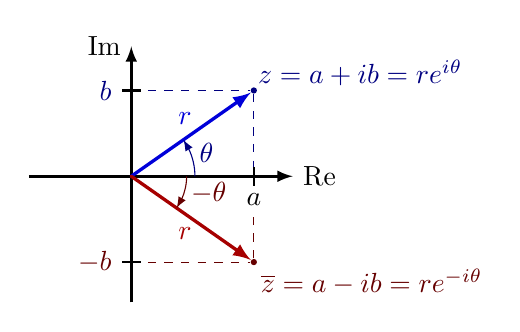
\begin{tikzpicture}
                \def\xmax{2.0}
                \def\ymax{1.6}
                \def\R{1.9}
                \def\ang{35}
                \coordinate (O) at (0,0);
                \coordinate (R) at (\ang:\R);
                \coordinate (-R) at (-\ang:\R);
                \coordinate (a) at ({\R*cos(\ang)},0);
                \coordinate (b) at (0,{\R*sin(\ang)});
                \coordinate (-b) at (0,{-\R*sin(\ang)});
                \node[fill=mydarkblue,circle,inner sep=0.8] (R') at (R) {};
                \node[fill=mydarkred,circle,inner sep=0.8] (-R') at (-R) {};
                \node[mydarkblue,above right=-2] at (R') {$z=a+ib=re^{i\theta}$};
                \node[mydarkred,below right=-1] at (-R') {$\overline{z}=a-ib=re^{-i\theta}$};
                \draw[dashed,mydarkblue]
                  (b) -- (R') --++ (0,{0.1-\R*sin(\ang)});
                \draw[dashed,mydarkred]
                  (-b) -- (-R') --++ (0,{\R*sin(\ang)-0.45});
                \draw[->,line width=0.9] (-0.65*\xmax,0) -- (\xmax+0.05,0) node[right] {Re};
                \draw[->,line width=0.9] (0,-\ymax) -- (0,\ymax+0.05) node[left] {Im};
                \draw[vector] (O) -- (R') node[pos=0.55,above left=-2] {$r$};
                \draw[vector,myred] (O) -- (-R') node[pos=0.55,below left=-2] {$r$};
                \draw pic[->,"$\theta$",mydarkblue,draw=mydarkblue,angle radius=23,angle eccentricity=1.24]
                  {angle = a--O--R};
                \draw pic[<-,"$-\theta$"{right=-1},mydarkred,draw=mydarkred,angle radius=20,angle eccentricity=1]
                  {angle = -R--O--a};
                %\tick{X}{90} node[scale=0.9,left=6,below right=-2] {$x = r\cos\theta$};
                \tick{a}{90} node[scale=1,below=-1] {$a$};
                \tick{b}{ 0} node[mydarkblue,scale=1,left] {$b$}; %r\sin\theta = 
                \tick{-b}{ 0} node[mydarkred,scale=1,left] {$-b$};
              \end{tikzpicture}
        \end{definition}

        \begin{proposition}
            \textbf{Propiedades:}
            Si $z,\ w\in \C$ entonces
            \begin{enumerate}
                \item $\overline{z+w}= \overline{z}+\overline{w}$,\quad $\overline{z\cdot w} = \overline{z}\cdot \overline{w}$
                \item $z=\overline{z} \Longleftrightarrow z\in\R$
            \end{enumerate}
        \end{proposition}
        
    \end{subsection}

\end{section}


\newpage

% ------------------------------------------------------------------------------
% Reference and Cited Works
% ------------------------------------------------------------------------------

% ------------------------------------------------------------------------------

\end{document}